\documentclass[english, 11pt, titlepage]{article}

\usepackage[utf8]{inputenc}    
\usepackage[english]{babel}
\usepackage[top=2.5cm, bottom=2.5cm, left=2.5cm, right=2.5cm]{geometry}
\usepackage{fancyhdr}
\usepackage{lastpage}
\usepackage{appendix}

%Path relative to the .tex file containing the \includegraphics command
\usepackage{graphicx}
\graphicspath{ {images/} }

\pagestyle{fancy}
\fancyhf{}
\rhead{(\thepage)}
\lhead{LP2A - Spring 2021}

% Clickable table of contents
\usepackage{hyperref}
\hypersetup{
    colorlinks,
    citecolor=black,
    filecolor=black,
    linkcolor=black,
    urlcolor=black
}

% Code + colors
\usepackage{listings}
\usepackage{color}

\definecolor{dkgreen}{rgb}{0,0.6,0}
\definecolor{gray}{rgb}{0.5,0.5,0.5}
\definecolor{mauve}{rgb}{0.58,0,0.82}

\lstset{frame=tb,
  language=Java,
  aboveskip=3mm,
  belowskip=3mm,
  showstringspaces=false,
  columns=flexible,
  basicstyle={\small\ttfamily},
  numbers=none,
  numberstyle=\tiny\color{gray},
  keywordstyle=\color{blue},
  commentstyle=\color{dkgreen},
  stringstyle=\color{mauve},
  breaklines=true,
  breakatwhitespace=true,
  tabsize=3
}

\begin{document}

    \begin{titlepage}
    \begin{center}
        \vspace*{1cm}
            
        \Huge
        \textbf{Programming a Ludo Game}
            
        \vspace{0.5cm}
        \LARGE
        Project report
            
        \vspace{1.5cm}
            
        \textbf{Florian CLOAREC} \\
        \textbf{Théo DURR}
        
        \vspace{1.5cm}
        
        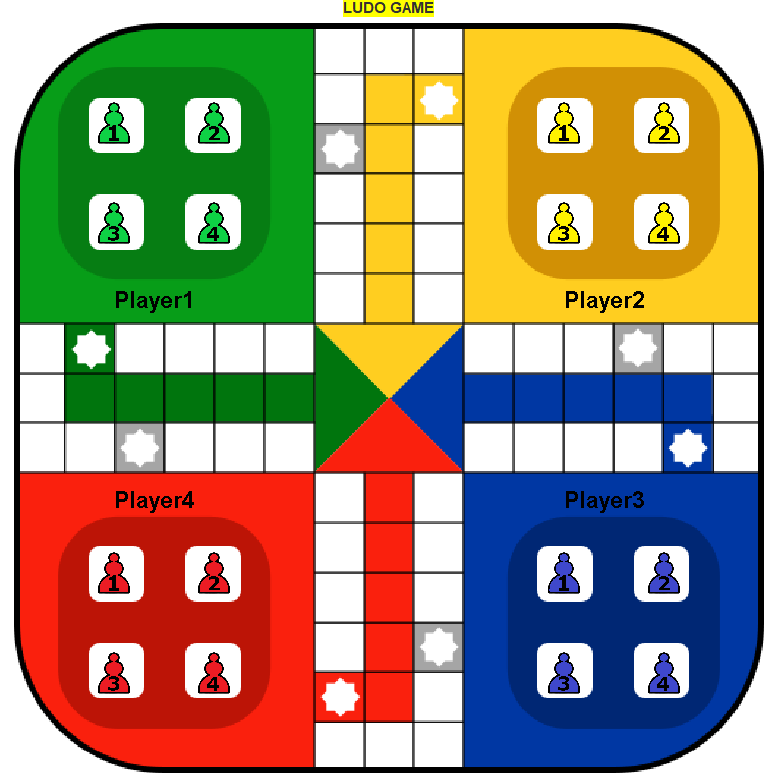
\includegraphics[width=0.45\textwidth]{titlepage.jpg}

        \vfill
                  
        
        \Large
        LP2A - Introduction to object conception and programming \\
        Spring 2021\\
        Université de Technologie de Belfort-Montbéliard\\
        \vspace{0.5cm}
        
\includegraphics[width=0.3\textwidth]{utbm_forword-2.jpg}
            
    \end{center}
\end{titlepage}

    \pagebreak
    \tableofcontents

    \pagebreak
    \section{Introduction}
    \subsection{Project Analysis}
    % Talk about UML, OOP programming
    First of all, we performed an analysis of the subject by defining, the behaviour, the constraints or even the signature of each class and represented all of this in an \textbf{UML Class Diagram}.
    \subsection{Organization}
    % Talk about task repartition, package organization, documentation
    \subsubsection{Tools used}
    % Talk about git, IntelliJ
    We also used some tools like IntelliJ Idea as IDE, for time saving tasks like compiling, creating packages, making unit tests, and so on. As a \textbf{Version Control System (VCS)}, we used \emph{Git}. It allowed us a better collaboration, a way to backup our files and, last but not least : It is a tool widely spread in the computer science jobs. So performing on this tool is a real benefit for the future.
    \begin{center}
        
\includegraphics[width=2cm]{IntelliJ_IDEA_Icon.svg.png}
        \hspace{2cm}
        
\includegraphics[width=2cm]{git.png}
    \end{center}

    Moreover, we decided to write this report in latex, as it is easier to insert some code, and mathematical formulas.
    \subsubsection{Documentation of the source files}
    As we used IntelliJ Idea, documenting the code was really simple. We trigger the snippet by typing \verb|/**|, then by pressing \verb|<Tab>| and it generates the documentation template, all we need to do is to fill in the description of the parameters and the return, and to provide a description of the function.

    \begin{lstlisting}
        // Example of documentation generation
        /**
        * PUT DESCRIPTION HERE
        * @param position PUT PARAMETER DESCRIPTION HERE
        * @return PUT RETURN DESCRIPTION HERE
        */
    \end{lstlisting}

    \section{The game components}
    This project is split into two main components : \emph{game engines} and \emph{graphical user interface (GUI)}. The engines are the core of the game. They ensure IAs are following certain rules, as well as player, who are restricted in their choices with the GUI by displaying only "rules friendly" moves. We will detail some of the functionnalities.

    Before explaining the engines, we need to talk about the components needed for it. They play a main role in the OOP. Yet, they are quite simple. For a summarized view of the structure, see APPENDIX X

    \subsection{The Players}
    The players are the entities playing the game. They have several actions such as moving a Piece, throw a dice, or pass. However, they are two types of player : real players (Humans) and Bots (Artificial Intelligence), their actions would be different, for instance when moving a piece. By following OOP principles, all the player types inherit from an abstract parent class called \verb|Player|. 
    \subsubsection{Humans}
    Humans are described in the child class \verb|Human|. The difference between them and AIs results in the actions with the board, such as throwing a dice, choosing the piece to move, as there is some GUI implemented in the class. Here is the code for the \verb|choosePiece| method :
    \begin{lstlisting}
    // Human.java
    public Piece choosePiece() {
        List<Piece> movablePiece = this.getMovablePieces();
        if (movablePiece.size() == 0) {
            JOptionPane.showMessageDialog(null, this.getName() + " : You can't move any piece, you have to pass");
            return null;
        } else {
            movablePiece.sort(new SortByBestMove());
            Collections.reverse(movablePiece);
            String[] stringMovablePiece = new String[movablePiece.size() + 1];

            for (int i = 0; i < movablePiece.size(); i++) {
                stringMovablePiece[i] = "" + movablePiece.get(i).getNumber();

            }
            stringMovablePiece[movablePiece.size()] = "pass";
            String result = (String) JOptionPane.showInputDialog(null, this.getName() + " : Choose the piece that you want move " + this.getDice().getValue() + " cases forward", this.getName() + " : Choose Piece", JOptionPane.QUESTION_MESSAGE, null, stringMovablePiece, stringMovablePiece[0]);

            if (result == null) {
                System.exit(1);
            }

            int intResult;
            try {
                intResult = Integer.parseInt(result);
            } catch (NumberFormatException e) {
                return null;
            }
            return this.getPieces()[intResult - 1];
        }
    }
    \end{lstlisting}
    We can see that there is some GUI code inside the \verb|Human| class. We found it was a good compromise between code organization and code efficiency.

    \subsubsection{Artificial Intelligences}
    Artificial Intelligences (AIs) work slightly different : there is no GUI code, as they are managed by the computer. So the work here was to implement the reflexion of the AI. As the main goal of this project was not to do machine learning, we simply implement a procedural set of \verb|if/else| statements in a separate java class:
    \begin{lstlisting}
    // SortByBestMove.java
    public class SortByBestMove implements Comparator<Piece> {
        @Override
        public int compare(Piece piece1, Piece piece2) {
            if (piece1 == null) {
                return -1;
            } else if (piece2 == null) {
                return 1;
            } else if (piece2.isAtStable() && !piece1.isAtStable()) {
                return -1;
            } else if (piece1.isAtStable() && !piece2.isAtStable()) {
                return 1;
            } else if (!piece1.isAtImmuneSquare() && piece2.isAtImmuneSquare()) {
                return 1;
            } else if (!piece2.isAtImmuneSquare() && piece1.isAtImmuneSquare()) {
                return -1;
            } else {
                return piece1.getPosition().getProgress() - piece2.getPosition().getProgress();
            }
        }
    }
    \end{lstlisting}

    \subsection{The Coordinates System}
    Each position object is composed of a color which is the color of the player and an integer "progress" which is the number of squares covered from the starting square. In the PositionConstant class, we make the link between the name of the important squares and the value of progress to which they correspond. Thus the stable is worth -1, the departure 0 and the arrival or Home is worth 57. Thanks to this system, the progression of each player on the game board is easy to manage, because it is enough to increment the number of squares you want to advance. But the problem arises when you want to compare the positions of the pieces of the other players, because each position is given in a base relative to each player represented by the color of this player. To do this we need to create a function that allows to convert a position from one color to another. To do this, using modular arithmetic and basic operations, we calculate the position in the new base (See \autoref{section:translating_coordinates}). Once this value has been calculated, the method creates a new Position object with this calculated value and the desired color.
    \subsection{The board}
    The board of the game is quite simple. It contains all the players (no matter which type they are), and a Dice. Its complexity only results in its constructor, which is depending of the gamemode (See \autoref{section:gamemodes}). The \verb|Board| class contains some methods, such as \verb|getPiecesAtCoordinates| :
    \begin{lstlisting}
        /**
        * Computes the pieces at given coordinates
        * @param position the position to check
        * @return List of piece if found, null either
        */
       public List<Piece> getPiecesAtCoordinates(Position position){
           List<Piece> result = new ArrayList<>();
           for (Player player : getPlayers()) {
               for (Piece piece : player.getPieces()) {
                   if (piece.getPosition().equals(position)) {
                       result.add(piece);
                   }
               }
           }
           if (result.isEmpty()) {
               return null;
           } else {
               return result;
           }
       }   
    \end{lstlisting}
    \subsubsection{The pieces \& the dice}

    \section{The game engines}
    They are 3 engines in total. Each engine is called depending of the gamemode. By following OOP principles, all the engines inherit from an abstract parent class called \verb|Engine|.
    \subsection{Managing collisions}
    Managing collisions is a central feature of the game, it ensure pieces go to the stable according to the rules of the game (and according to the \autoref{fig:logigram})
    
    This feature is required by the rules of the game, we implemented it, but with more time, we could have tested it. We might expect some bugs.
    % Implemented, but not tested

    \subsection{Gamemodes}
    \label{section:gamemodes}

    \subsubsection{4 Artificial Intelligences}
    This gamemode was not required in the specifications, but we made it for \emph{experimental purposes}. It allowed us to check if everything was working properly without having a GUI. The four players are AIs and are playing by following the rules.
    \subsubsection{4 Players}
    This gamemode unlieve the entire potential of the GUI, by allowing four players to play in the same time on the same computer. Each player plays one after the other.

    \subsubsection{1 Player versus 3 Artificial Intelligences}

    \section{The graphical user interface (GUI)}
    \subsection{Aspect of the game}
    \subsection{Interactions with the user}
    \subsection{Translating relatives coordinates in absolute coordinates}

    \section{Conclusion}
    \subsection{Improvements paths}
    \subsection{Benefits of this project}
    \label{section:translating_coordinates}

    \pagebreak
    \appendix
    \appendixpage
    \addappheadtotoc
    \section{Unified Modeling (UML) Diagram}
    \subsection{Engine}

    \pagebreak
    \section{Simplified algorithm}
    \label{fig:algorithm}
    \begin{figure}[h]
        \centering
        \vspace{0.3cm}
        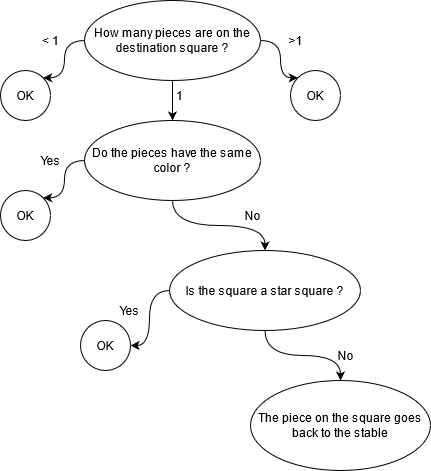
\includegraphics{Logigram.png}
    \end{figure}
    
\end{document}